%-----------------------------------------------------------------------------
%	 Casos de Uso 
%-----------------------------------------------------------------------------

\lhead[\thepage]{Casos de Uso \thechapter. \rightmark}
\rhead[Casos de Uso \thechapter. \leftmark]{\thepage}

%	Capitulo 8: Casos de Uso
\chapter{Casos de Uso}
\markboth{Casos de Uso}{Casos de Uso}
Para la solución prevista, especificamente los componentes de que requieren comunicarse usando MQTT como protocolo se establece el caso de uso :

\begin{figure}[htb]
\centering
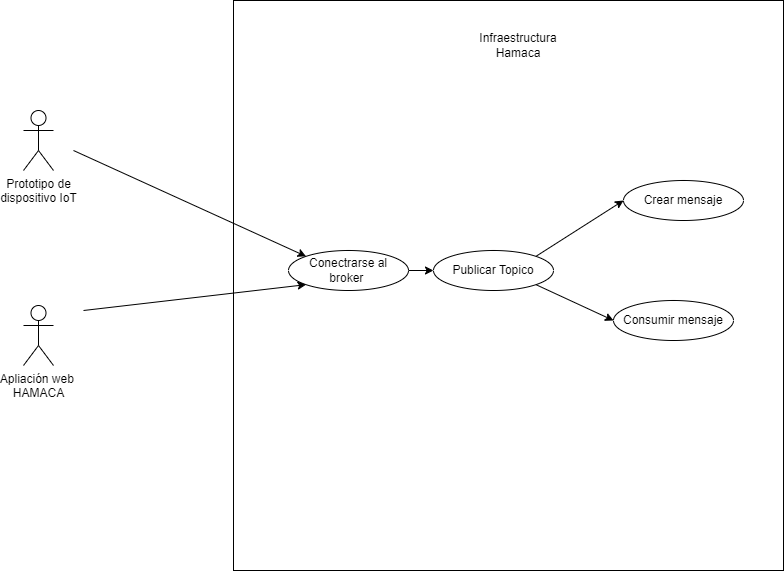
\includegraphics[scale=0.35]{./Figuras/caso_de_uso_mqtt.png}
\caption{Diagrama de caso de uso para la comuniación MQTT}
\label{fig:caso_de_uso_mqtt}
\vspace*{-10pt}
\end{figure}

A continuación se explica cada acción dentreo del caso de uso:
\begin{itemize}
\item el tal
\end{itemize}

\begin{figure}[htb]
\centering
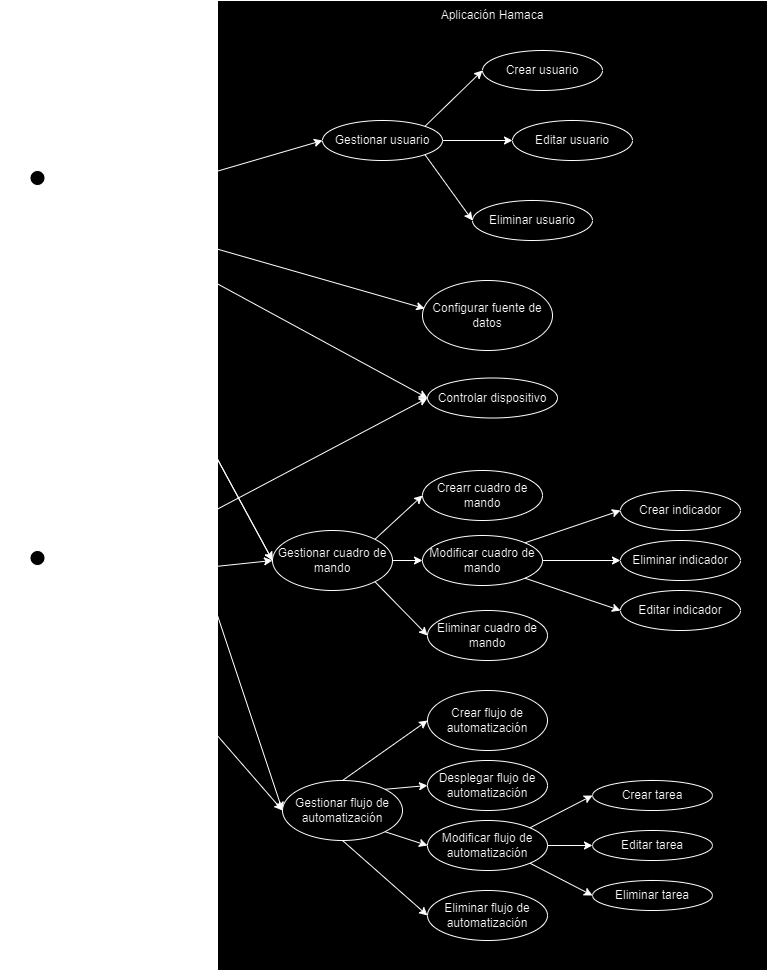
\includegraphics[scale=0.35]{./Figuras/caso_de_uso.png}
\caption{Diagrama de caso de uso para la apliación web HAMACA}
\label{fig:caso_de_uso}
\vspace*{-10pt}
\end{figure}


\section{Laboratorios de Investigación y Desarrollo}
\lhead[\thepage]{\thesection. Laboratorios de Investigación y Desarrollo}
hue
\subsection{Entornos Académicos}
hue
\subsection{Entornos Industriales}
hue

\section{Ambientes Domésticos y Oficinas}
\lhead[\thepage]{\thesection. Ambientes Domésticos y Oficinas}
hue
